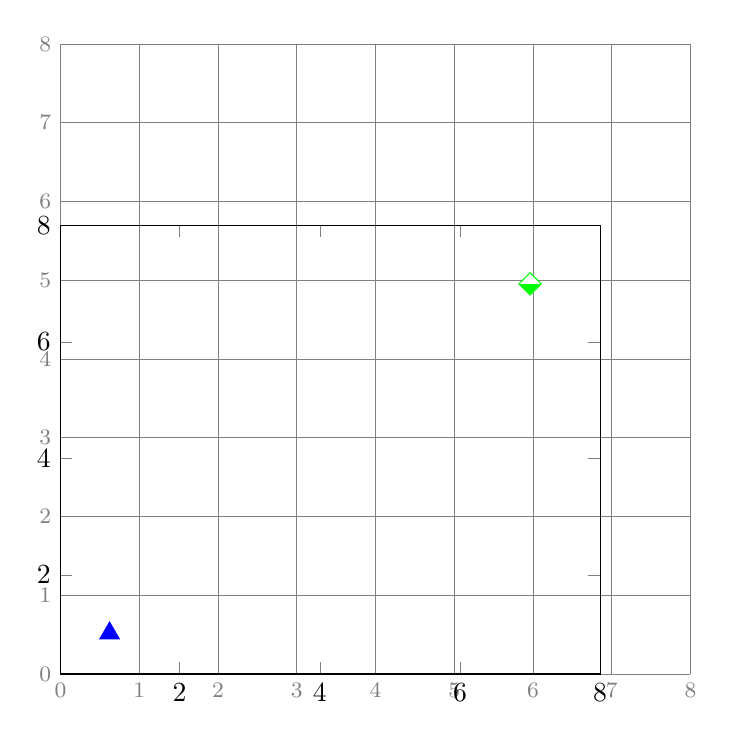
\begin{tikzpicture} [>=latex]
 \draw [help lines] (0,0) grid (8, 8);
 \foreach \x in {0,1,...,8}
   \draw [help lines] (\x,0) node [below,%
          font=\footnotesize] {$\x$} -- (\x,0);
\foreach \y in {0,1,...,8}
   \draw [help lines] (0,\y) node [left,%
          font=\footnotesize] {$\y$} -- (0,\y);
\begin{axis}[
    domain=0:10,
    xmax=8,
    ymax=8,
    view={0}{90},
]
%\def\ka{2000}
%\def\length{sqrt(-\ka((\pstart-\pend)^2+(\pstart-\pend)^2))}
\def\pstart{(1,1)}
\def\pend{(7,7)}
  %define robot
  \addplot+[mark=triangle*, mark options={%
  scale=2}]coordinates{(1,1)};
  %define goal
  \addplot+[mark=halfsquare*,mark options={%
        scale=2,fill=green,draw=green
    }]coordinates{(7,7)};

\def\eq{ -3(-(x*x+y*y)/2) };  
%\addplot3[blue,/pgfplots/quiver,
%    quiver/\length=y,
%    quiver/\length=x,
%%    %quiver/w=0,
%   quiver/scale arrows=0.1,
% -stealth,samples=10] {1};
%]

%\addplot3 [gray, quiver={u={\pend/\eq}, v={\pend/\eq}, scale arrows=0.2, every arrow/.append style={-latex}}] (x,y,0);
\end{axis}
 \end{tikzpicture}